\documentclass[border=5pt, multi, tikz]{standalone}
\usepackage{import}
\usepackage{amsmath}
\usepackage{amssymb}
\usetikzlibrary{positioning, arrows.meta, shapes.geometric, calc, fit, backgrounds}

% 定义颜色
\definecolor{cnncolor}{RGB}{220, 20, 60}          % 红色 - CNN
\definecolor{tcncolor}{RGB}{255, 140, 0}          % 橙色 - TCN
\definecolor{fusioncolor}{RGB}{70, 130, 180}      % 钢蓝 - Fusion
\definecolor{inputcolor}{RGB}{100, 149, 237}      % 浅蓝 - Input
\definecolor{outputcolor}{RGB}{60, 179, 113}      % 绿色 - Output
\definecolor{metacolor}{RGB}{147, 112, 219}       % 紫色 - Meta

\begin{document}
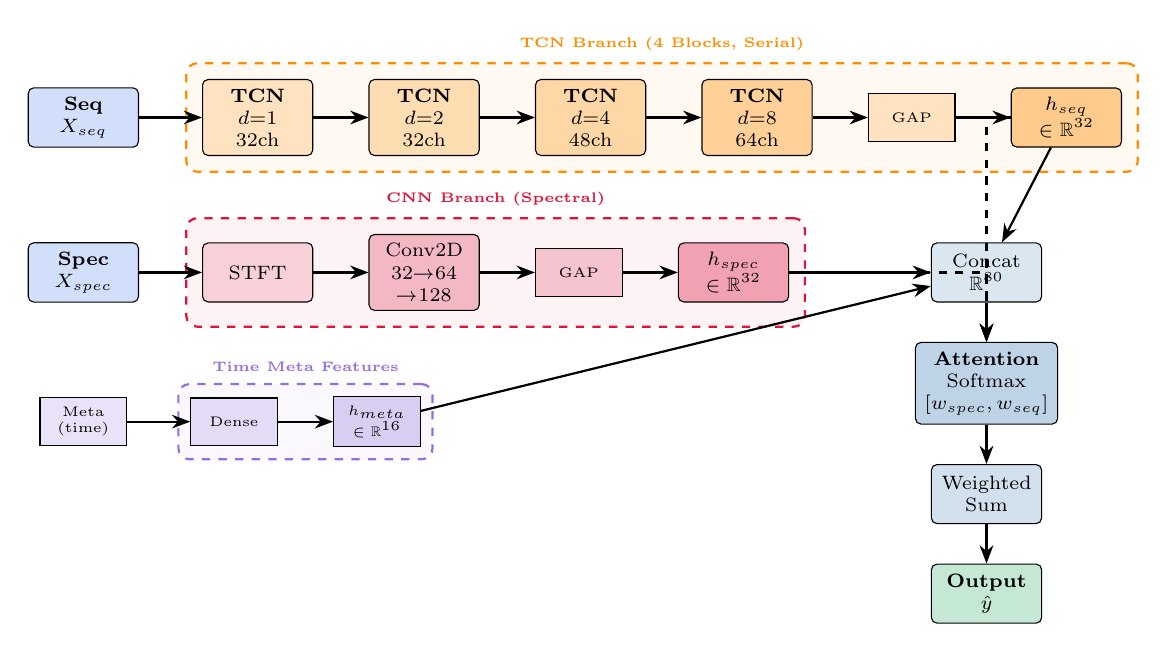
\begin{tikzpicture}[
    node distance=0.4cm and 0.7cm,
    box/.style={rectangle, draw, minimum width=1.4cm, minimum height=0.75cm, align=center, font=\scriptsize, rounded corners=2pt},
    smallbox/.style={rectangle, draw, minimum width=1.1cm, minimum height=0.6cm, align=center, font=\tiny},
    arrow/.style={-Stealth, thick},
    dashedarrow/.style={-Stealth, thick, dashed},
]

% ============ 输入层 (左侧) ============
\node[box, fill=inputcolor!30] (input_spec) {\textbf{Spec}\\$X_{spec}$};
\node[box, fill=inputcolor!30, above=1.2cm of input_spec] (input_seq) {\textbf{Seq}\\$X_{seq}$};
\node[smallbox, fill=metacolor!20, below=1.2cm of input_spec] (input_meta) {Meta\\(time)};

% ============ CNN分支 (上层) ============
\node[box, fill=cnncolor!20, right=0.8cm of input_spec] (stft) {STFT};
\node[box, fill=cnncolor!30, right=of stft] (conv2d) {Conv2D\\32→64\\→128};
\node[smallbox, fill=cnncolor!25, right=of conv2d] (gap_cnn) {GAP};
\node[box, fill=cnncolor!40, right=of gap_cnn] (h_cnn) {$h_{spec}$\\$\in \mathbb{R}^{32}$};

% ============ TCN分支 (中层,4层串行) ============  
\node[box, fill=tcncolor!25, right=0.8cm of input_seq] (tcn1) {\textbf{TCN}\\$d{=}1$\\32ch};
\node[box, fill=tcncolor!30, right=of tcn1] (tcn2) {\textbf{TCN}\\$d{=}2$\\32ch};
\node[box, fill=tcncolor!35, right=of tcn2] (tcn3) {\textbf{TCN}\\$d{=}4$\\48ch};
\node[box, fill=tcncolor!40, right=of tcn3] (tcn4) {\textbf{TCN}\\$d{=}8$\\64ch};
\node[smallbox, fill=tcncolor!25, right=of tcn4] (gap_tcn) {GAP};
\node[box, fill=tcncolor!45, right=of gap_tcn] (h_tcn) {$h_{seq}$\\$\in \mathbb{R}^{32}$};

% ============ Meta分支 (下层) ============
\node[smallbox, fill=metacolor!25, right=0.8cm of input_meta] (meta_dense) {Dense};
\node[smallbox, fill=metacolor!35, right=of meta_dense] (h_meta) {$h_{meta}$\\$\in \mathbb{R}^{16}$};

% ============ 融合层 (右侧) ============
\node[box, fill=fusioncolor!20, right=1.8cm of h_cnn] (concat) {Concat\\$\mathbb{R}^{80}$};

\node[box, fill=fusioncolor!35, below=0.5cm of concat, minimum height=1cm] (attention) {\textbf{Attention}\\Softmax\\$[w_{spec}, w_{seq}]$};

\node[box, fill=fusioncolor!25, below=0.5cm of attention] (fused) {Weighted\\Sum};

% ============ 输出 ============
\node[box, fill=outputcolor!30, below=0.5cm of fused] (output) {\textbf{Output}\\$\hat{y}$};

% ============ 箭头 ============
% 输入→各分支
\draw[arrow] (input_spec) -- (stft);
\draw[arrow] (input_seq) -- (tcn1);
\draw[arrow] (input_meta) -- (meta_dense);

% CNN分支流程
\draw[arrow] (stft) -- (conv2d);
\draw[arrow] (conv2d) -- (gap_cnn);
\draw[arrow] (gap_cnn) -- (h_cnn);

% TCN分支流程 (串行4层)
\draw[arrow] (tcn1) -- (tcn2);
\draw[arrow] (tcn2) -- (tcn3);
\draw[arrow] (tcn3) -- (tcn4);
\draw[arrow] (tcn4) -- (gap_tcn);
\draw[arrow] (gap_tcn) -- (h_tcn);

% Meta分支流程
\draw[arrow] (meta_dense) -- (h_meta);

% 3个特征→Concat
\draw[arrow] (h_cnn) -- (concat);
\draw[arrow] (h_tcn) -- (concat);
\draw[arrow] (h_meta) -- (concat);

% Concat→Attention (h_cnn和h_tcn通过虚线影响attention)
\draw[arrow] (concat) -- (attention);
\draw[dashedarrow] (h_cnn) -| (attention);
\draw[dashedarrow] (h_tcn) -| (attention);

% Attention→输出
\draw[arrow] (attention) -- (fused);
\draw[arrow] (fused) -- (output);

% ============ 背景框 ============
\begin{pgfonlayer}{background}
    % CNN分支背景
    \node[draw=cnncolor, thick, dashed, rounded corners, 
          fit={(stft) (conv2d) (gap_cnn) (h_cnn)}, 
          fill=cnncolor!5, inner sep=0.2cm] (cnn_box) {};
    \node[above=0.02cm of cnn_box, font=\tiny\bfseries, text=cnncolor] {CNN Branch (Spectral)};
    
    % TCN分支背景
    \node[draw=tcncolor, thick, dashed, rounded corners, 
          fit={(tcn1) (tcn2) (tcn3) (tcn4) (gap_tcn) (h_tcn)}, 
          fill=tcncolor!5, inner sep=0.2cm] (tcn_box) {};
    \node[above=0.02cm of tcn_box, font=\tiny\bfseries, text=tcncolor] {TCN Branch (4 Blocks, Serial)};
    
    % Meta分支背景
    \node[draw=metacolor, thick, dashed, rounded corners, 
          fit={(meta_dense) (h_meta)}, 
          fill=metacolor!5, inner sep=0.15cm] (meta_box) {};
    \node[above=0.02cm of meta_box, font=\tiny\bfseries, text=metacolor] {Time Meta Features};
\end{pgfonlayer}

\end{tikzpicture}
\end{document}
